\\
$g$ is a \emph{subgradient} of $f$ (not necessarily convex) at $x$ if 
\\
\begin{center}
$\forall y  \qquad f(y) \geq f(x)+ g^T(y-x)  $
\end{center}


%Include figure
\begin{center}
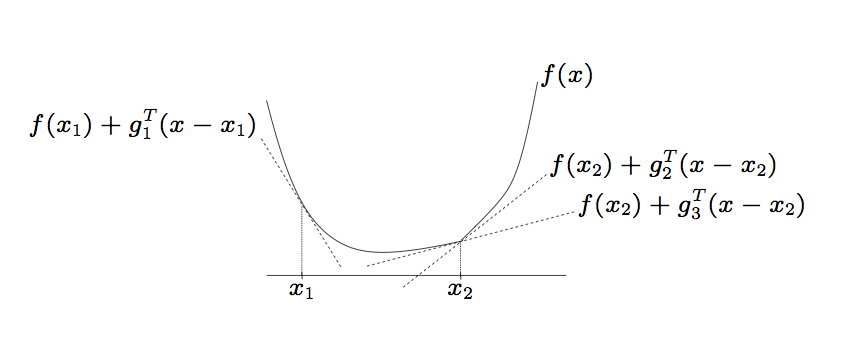
\includegraphics[width=0.8\textwidth]{subgrad_figure}
\end{center}


($g_1$ is a subgradient at $x_1$; $g_2$ and $g_3$ are subgradients at
$x_2$)%Probably unnecessary..


